\section{Gradiente Descendente}

Se trata de un algoritmo de aprendizaje iterativo clásico, basado en el método de optimización para funciones lineales de Cauchy. Haskell Curry lo estudió por primera vez para optimización no lineal en 1944 \cite{Curry1944GDNoLin}, siendo ampliamente usado a partir de las décadas de los 1950-1960. Actualmente se trata de la estrategia de entrenamiento de modelos más ampliamente usada, especialmente en los modelos de aprendizaje profundo, siendo la estrategia que mejores resultados consigue en cuanto a capacidad de generalización de los modelos y eficiencia computacional gracias a su aplicación a través del algoritmo de BP. Sin embargo a nivel práctico no se usa en su versión original, sino que a lo largo del tiempo han ido surgiendo numerosas modificaciones con el objetivo de mejorar el algoritmo en diversos ámbitos: aumento de la estabilidad y la velocidad de convergencia, reducción computacional del entrenamiento, capacidad de evitar mínimos locales, etc. Estos métodos modificados del original se conocen como optimizadores. La literatura en este sentido es extensa, y aunque es bastante claro que el gradiente descendente sigue siendo la mejor estrategia de optimización de parámetros de un modelo de forma general, la elección del algoritmo de optimización concreto y de su ajuste depende del problema concreto que estemos tratando y generalmente se realiza de manera experimental. 

Debemos ver que el entrenamiento de los modelos, en su gran mayoría, está intrínsecamente ligado a la optimización, específicamente a la minimización de la función de coste $C$. Este no es un problema sencillo, y como se ha mencionado antes se trata de un problema NP-Completo, por tanto de existir algoritmos exactos estos requieren demasiado coste computacional como para utilizarlos en la práctica, por lo que se buscan estrategias aproximadas como el descenso de gradiente para obtener buenas soluciones en un tiempo asequible. 

Otros factores a tener en cuenta son la necesidad de escapar de óptimos locales, aún no conociendo de manera explícita la función de error; y la generalización: no es  importante únicamente obtener un error bajo en el entrenamiento sino que se mantenga cuando usamos datos de entrada nuevos, ya que nuestro objetivo es ser capaces de encontrar patrones que podamos aplicar en situaciones nuevas y no ajustar el modelo a unos datos dados.

\subsection{Gradiente descendente de Cauchy}

Procedemos a describir el método original de descenso de gradiente, propuesto en 1847 por Augustin-Louis Cauchy \cite{CauchyGD}. Es una versión más primitiva y limitada que sus desarrollos posteriores pero que nos permite obtener de forma más sencilla una visión de su funcionamiento. 

Fijamos $f:\mathbb{R}^n \rightarrow \mathbb{R}$ una función continua que no toma valores negativos. Las notamos por $x= \left ( x_1,\ldots,x_n \right ) \in \mathbb{R}^n$. Si queremos encontrar los valores de $x_1,\ldots,x_N$ que verifican $f(x_1,\ldots,x_n)=0$, que suponemos que existen, bastará con hacer decrecer indefinidamente los valores de la función $f$ hasta que sean muy cercanos a $0$. 

Fijamos ahora unos valores concretos $x_0 \in \mathbb{R}^n$, $u=f(x_0)$,\\ $Du= \left ( D_{x_1}u, D_{x_2}u, \ldots, D_{x_n}u \right )$ y $\epsilon >0$ con $\epsilon \in \mathbb{R}^n$. Si tomamos $x_0'=x_0+\epsilon$ tendremos:
$$f(x_0')= f(x_0 + \epsilon) = u + \epsilon Du$$

Sea ahora $\eta >0$, tomando $\epsilon= - \eta Du$ con la fórmula anterior tenemos: 

$$f(x_0') = f(x_0 + \epsilon) = u - \eta \sum_{i=1}^{n}(D_{x_i}u)^2$$

Por tanto hemos obtenido un decremento en el valor de la función $f$ modificando los valores de sus variables en sentido contrario al gradiente, para $\eta$ suficientemente pequeño. El objetivo de la estrategia es repetir esta operación hasta que se desvanezca el valor de la función $f$.




\subsection{Gradiente descendente en el entrenamiento de modelos}

En el caso del aprendizaje de modelos la función que debemos minimizar es la función de coste $C$, que efectivamente es continua por ser composición de funciones continuas, como se verá más adelante. Esta función no toma valores negativos. Como no podemos realizar un cálculo continuo para comprobar con qué valores de $\eta$ la función decrece, lo hacemos de manera iterativa, y a este $\eta$ lo llamamos ratio de aprendizaje o más comúnmente \textit{learning rate}. 

En el proceso de entrenamiento de un modelo lo que hacemos es aplicar la idea anterior de manera iterativa en lugar de encontrar un $\eta$ que minimice en un paso, para ir moviéndonos a puntos de menor valor de la función de coste. Si $C(W)$ es la función de coste del modelo y $W$ representa los parámetros del modelo, entonces la regla de actualización iterativa del descenso del gradiente es la siguiente:

\begin{equation}\label{eq:GD}
W_{t+1}=W_t - \eta \nabla C(W)
\end{equation}

En su descripción original, el gradiente se calcula usando todos los datos de entrenamiento, pero en versiones posteriores se propone dividir el conjunto de entrenamiento en varios subconjuntos disjuntos, denominados lotes. Cada vez que se calcula el gradiente se actualizan los pesos, y denominamos a esto una iteración. Cada vez que se usan todos los datos de entrenamiento para calcular el gradiente, ya sea tras una sola iteración usando todo el conjunto de entrenamiento o varias si dividimos en lotes, lo denominamos época.



\subsubsection{Estrategias de gradiente descendente} \label{sec:estrategias}

En base a los lotes en que dividamos el conjunto de entrenamiento tenemos varios tipos de gradiente descendente \cite{GoodFellowBook}.

\begin{itemize}
    \item \textbf{Batch Gradient Descent} (BGD): tenemos un único lote, cada iteración se corresponde con una época. Calculamos el gradiente usando todo el conjunto de entrenamiento. Esto ofrece un comportamiento mejor estudiado a nivel teórico, con más resultados demostrados; pero aumenta mucho el coste computacional del entrenamiento hasta el punto que lo vuelve demasiado lento para ser usado en la práctica.

    \item \textbf{Stochastic Gradient Descent} (SGD): Actualiza los pesos calculando el gradiente con sólo un elemento del conjunto de entrenamiento. Cada época tiene tantas iteraciones como número de elementos haya en el conjunto de entrenamiento. Esta estrategia introduce ruido en el entrenamiento ya que el gradiente se calcula de una manera aproximada, aunque esto tiene un efecto positivo ya que al provocar más irregularidad en la trayectoria de convergencia es más probable poder escapar mínimos locales. Además es más eficiente computacionalmente que el anterior y converge más rápido en la práctica.

    \item \textbf{Mini-Batch Gradient Descent} (MBGD): Se divide el conjunto de entrenamiento en M lotes de tamaño fijo, y se calcula el gradiente con cada lote, por lo que habrá M iteraciones en cada época. Se consigue una aproximación del gradiente con menos error al usar más datos para su cálculo y además se siguen manteniendo las propiedades que veíamos en la anterior estrategia. Es más eficiente que la anterior al conllevar menos actualizaciones de pesos. Es prácticamente la única estrategia utilizada en la realidad ya que ofrece la mayor eficiencia computacional, estabilidad y rapidez en la convergencia.
\end{itemize}

Aunque la política para computar el gradiente sea distinta en estos 3 tipos, los englobaremos dentro de lo que denominaremos el algoritmo de gradiente descendente original, ya que como veremos más adelante, existen varias modificaciones del algoritmo que aportan mejoras a través de modificar la regla de actualización de los pesos y no solo la cantidad de datos con la que se aproxima el gradiente.

\subsubsection{\textit{Learning rate}}

El elemento $\eta$ que observamos en la ecuación \ref{eq:GD} del gradiente descendente se denomina \textit{learning rate} y lo usamos para controlar la convergencia reduciendo el efecto de la magnitud del gradiente en la actualización de los parámetros. Este valor es positivo y situado en la práctica alrededor de 0.01 y 0.001 usualmente, aunque para su elección conviene realizar un análisis teórico previo o realizar pruebas prácticas (mucho más común) para elegir un valor adecuado. Este tipo de parámetros, que no son parte del modelo sino del algoritmo de aprendizaje, se denominan hiperparámetros. Dependiendo del tipo de algoritmo o modificación del mismo que usemos habrá diferentes hiperparámetros, siendo el \textit{learning rate} el más importante de manera general, ya que de su valor dependerá la convergencia del algoritmo, pudiendo hacer que converja demasiado lento o que directamente diverja, como podemos observar en la figura \ref{fig:lr} o en resultados sobre la convergencia en la sección \ref{sec:convergencia}.

En cuanto a la selección de los hiperparámetros, no se enfoca como un problema donde se busque el óptimo de estos valores ya que la mayoría no son tan decisivos en la convergencia como el \textit{learning rate}, y se ofrecen valores teóricos en sus papers de presentación que funcionan bien en casos generales. Si bien la convergencia es sensible a los valores iniciales de estos hiperparámetros que se tratan de optimizar a nivel experimental a través del ensayo y error, aunque no se dedican excesivos recursos computacionales a esta búsqueda, invirtiéndose por el contrario en el entrenamiento.



\begin{figure}
    \centering
    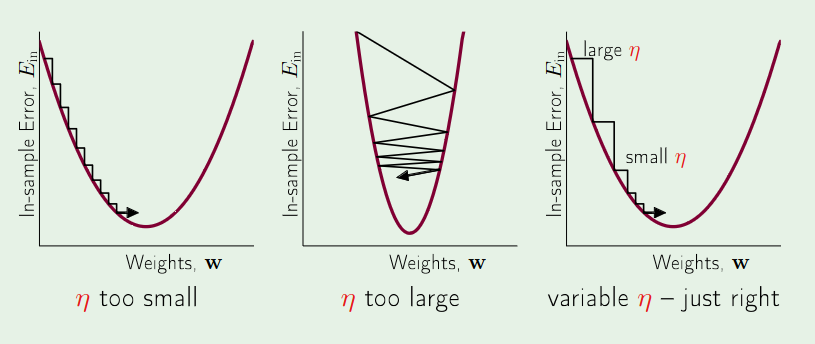
\includegraphics[width=0.5\linewidth]{Plantilla_TFG_latex//imagenes//Mat//GD/lr.png}
    \caption{Visualización de cómo afecta el \textit{learning rate} según su adecuación al problema. Imagen obtenida del curso de Caltech \footnote{https://home.work.caltech.edu/slides/slides09.pdf}, tema 9 diapositiva 21}
    \label{fig:lr}
\end{figure}

Una táctica habitual es usar una política de \textit{learning rate} que decrezca conforme avanza el entrenamiento, de manera que el algoritmo avance con pasos más grandes cuando aún está lejos del óptimo, con un objetivo explorador, y con pasos más pequeños cuando se va acercando, con un objetivo explotador, procurando una convergencia más estable. \cite{GoodFellowBook}. Otro enfoque común es también tener un vector de \textit{learning rate} en lugar de un solo escalar, teniendo un valor para cada peso del modelo. 





\subsection{Subgradientes} \label{sec:subgrad}

Con el objetivo central de calcular el gradiente es lógico pensar que necesitamos ciertas condiciones de diferenciabilidad, aunque sean mínimas, para poder calcular el gradiente que necesitamos. Podemos pensar en un modelo como una composición de la suma y producto de operaciones lineales con operaciones no lineales (funciones de activación), y componiendo ésta con la función de coste del modelo obtendríamos la función $f: X \times \Omega \times Y \rightarrow \mathbb{R^+}$, que recibe los pesos del modelo, los datos de entrada y sus etiquetas correctas para proporcionar el error del modelo. Esta es la función que necesitaríamos que fuera diferenciable. Las operaciones lineales preservan la diferenciabilidad, y la composición de funciones diferenciables es diferenciable por lo que si la función de pérdida y las funciones de activación son diferenciables, no tendremos ningún problema a la hora de calcular el gradiente.

Las funciones de coste son diferenciables de manera general, y la más común para problemas de clasificación es \textit{CrossEntropyLoss}, mientras que para regresión son comunes el error cuadrático medio y el error absoluto medio.

\begin{itemize}

    \item \textbf{ECM:} $\frac{1}{N} \sum_{i=1}^N \left (y_i - \hat{y} \right ) ^2$ 

    \item \textbf{EAM:} $\frac{1}{N} \sum_{i=1}^N \lvert y_i - \hat{y} \rvert$ 	

    \item \textbf{\textit{CrossEntropyLoss}:} $  - \sum_c \hat{y_c} log(\frac{e^{y_c}}{\sum_{c'=1}^C e^{y_{c'}}})$
\end{itemize}

 Donde $N$ es el número de datos, $\hat{y}_i$ es el valor real del dato $i$, que en ECM será un escalar, y en clasificación binaria será 0 ó 1; $y_c$ es el valor predicho por el modelo, $\hat{y}_{c}$ es la etiqueta real de la clase $c$, que valdrá 1 en caso de que el dato pertenece a la clase $c$ y 0 en caso contrario; y $y_{c}$ es el predicho por el modelo. 


Hasta el año 2010, las funciones de activación más comunes para las capas ocultas eran la función sigmoide y la tangente hiperbólica. Estas funciones son diferenciables por lo que su uso no suponía ningún problema en la aplicación del descenso de gradiente. Sobre ese año se empezó a popularizar la función de activación ReLU (Rectified Linear Unit), gracias a su simplicidad, reducción de coste computacional y su aparición en modelos ganadores de competiciones de ImageNet como AlexNet en 2012. Desde entonces esta función, junto a algunas de sus variantes que aparecen en la figura \ref{fig:3.ReLU} son ampliamente usadas y con buenos resultados. Sin embargo salta a la vista que esta función no es diferenciable.


\begin{figure}
    \centering
    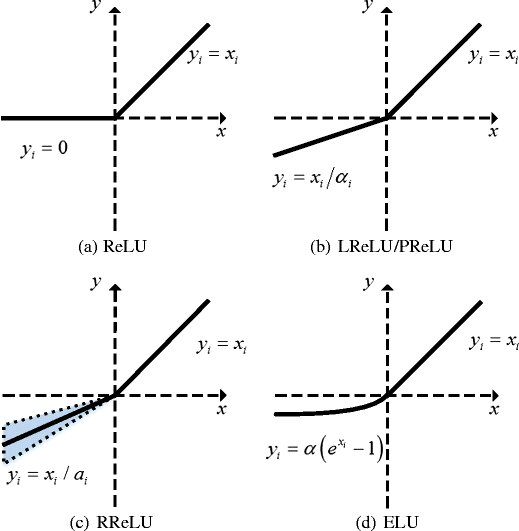
\includegraphics[width=0.5\linewidth]{3ReLU&oth.jpg}
    \caption{Función ReLU y algunas de sus variantes más usadas como funciones de activación.\footnote{https://www.researchgate.net/publication/319438080\_A\_novel\_softplus\_linear\_unit\_for\_deep\_convolutional\_neural\_networks}}
    \label{fig:3.ReLU}
\end{figure}



Vamos a presentar entonces el concepto de subgradiente junto con algunas de sus propiedades, obtenidas de \cite{convexSubgrad}, para ver que será una extensión del gradiente que nos permitirá usar el método de gradiente descendente con funciones que no sean diferenciables en algunos puntos pero que sí sean subdiferenciables.

\begin{definicion}[Subgradiente]
     Sea $A \subset \mathbb{R}^n$ y $f:A \rightarrow \mathbb{R}$, $g \in \mathbb{R}^n$ es un subgradiente de $f$ en $a \in A$ si $\forall y \in U_a$ entorno de $a$ se tiene:

    $$f(a)-f(y) \leq g^T(a-y)$$
    El conjunto de los subgradientes de $f$ en x se denota por $\partial f(a)$. Si existe el subgradiente de $f$ en a, decimos que $f$ es subdiferenciable en $a$.
\end{definicion}

Necesitamos también un comportamiento similar al de las funciones diferenciables, en particular necesitamos que las funciones subdiferenciables se preserven a través de las operaciones de suma, multiplicación por escalares y composición.

\begin{enumerate}

	\item{\textbf{Multiplicación escalar no negativa}: $\partial (af) = a \cdot \partial f , a\geq0$
	
	Por definición $g$ es un subgradiente de $f$ en $x_0$ si:
	
	$$f(x) \geq f(x_0) + g^T(x-x_0), \quad \forall x \in dom(f).$$

	Multiplicando la desigualdad por $c \geq 0$:

	$$cf(x) \geq cf(x_0) + cg^T(x-x_0), \quad \forall x \in dom(f).$$

	Por tanto $cg$ es un subgradiente de $h(x)=cf(x)$ en $x_0$.

	}
	
	\item{ \textbf{Suma}: $\partial (f_1+f_2) = \partial f_1 + \partial f_2$

	Sea $g_1$ un subgradiente de $f_1$ y $g_2$ un subgradiente de $f_2$, considerando el punto $x_0$, por definición tenemos:

	$$f_1(x) \geq f_1(x_0) + g_1^T(x-x_0), \quad x \in dom(f),$$

	$$f_2(x) \geq g_2(x_0) + g_2^T(x-x_0), \quad x \in dom(g).$$

	Sumamos las dos desigualdades para obtener que $g_1 + g_2$ es un subgradiente de $f_1 + f_2$:

	$$f_1(x) + f_2(x) \geq f_1(x_0) + f_2(x_0) + \left ( g_1 + g_2 \right ) ^T \left ( x - x_0 \right ).$$


	}
	
	\item{ \textbf{Composición afín}: Si $h(x)=f(Ax + b) \Rightarrow \partial h(x)= A^T \partial f(Ax+b)$
	
	$g$ es un subgradiente de $f$ en $y_0$:
	
	$$f(y) \geq f(y_0) + g^T(y-y_0), \quad \forall y \in dom(f).$$

	Tomamos $y=Ax + b$ y por tanto $y_0= Ax_0 + b$. Sustituyendo:

	$$f(Ax + b) \geq f(Ax_0 + b) + g^T(Ax + b - (Ax_0 + b)),$$

	$$h(x)=f(Ax+b) \geq h(x_0) + g^TA(x-x_0).$$

	Por tanto $A^Tg$ es un subgradiente de $h(x)=f(Ax+b)$ en $x_0$.

	}
	
\end{enumerate}


Tenemos que comprobar que el subgradiente extiende al gradiente, es decir, que cuando existe gradiente entonces existe un único subgradiente y coincide con él. Además hay funciones que no son diferenciables pero sí subdiferenciables. Esto último se hace evidente con el ejemplo anterior de la función ReLU. Vamos a demostrar por tanto que si $f: X \subseteq \mathbb{R}^n \rightarrow \mathbb{R}^m$ es diferenciable en el punto $x\in X$ entonces  $\partial f(x)= \left \{ \nabla f(x) \right \}$.

Como $f$ es diferenciable en $x$, existe un entorno $U_x$ de $x$ donde el gradiente satiface 

$$  f(y) = f(x) + \nabla f(x)^T(y-x) + o(\|y-x \|) \forall y \in U_x.$$

Por tanto tenemos

$$ f(y) \geq f(x) + \nabla f(x)^T(y-x), \forall y \in U_x.$$

Es decir que el gradiente de $f$ en $x$ es también un subgradiente de $f$ en $x$. Tenemos que $\nabla f(x) \in \partial f(x)$, nos queda demostrar que es único. Para ello vamos a suponer que existe otro subgradiente de $f$ en $x$, $g \in \partial f(x)$. Sea $y=x+tw$, definimos la función

$$\phi(t)=f(y)-f(x)- g^T(y-x) = f(x+tw) -f(x) - g^T(tw) \geq 0$$

donde se ha usado que $g \in \partial f(x)$. Derivamos la función para obtener $\phi'(t) = \nabla f(x)^Tw - g^Tw$. Vemos que para $t=0$ se tiene que $\phi(0)=0$, con lo que hay un mínimo en ese punto. Tenemos por tanto que $\phi'(0)=0$ o equivalentemente $\nabla f(x)^Tw=g^Tw$. Como $w$ es arbitrario, concluimos que $g=\nabla f(x)$. Como el gradiente es un subgradiente, y todo subgradiente coincide con él, se tiene que es único, $\partial f(x) = \left \{ \nabla f(x) \right \}$. 



Vamos ahora a presentar una proposición que relaciona los subgradientes con las funciones convexas, las cuales están muy ligadas a la convergencia del gradiente descendnte. Para ello primero vamos a definir lo que es un conjunto convexo, ya que resulta elemental tanto en esta sección como en la siguiente y usaremos este concepto para desarrollar otros a partir de él.


\begin{definicion}[Conjunto convexo]
    Un subconjunto $E$ de un espacio vectorial $X$ es convexo cuando, para cualesquiera dos puntos de $E$, el segmento que los une está contenido en $E$:

    $$x,y \in E \Rightarrow \left \{ (1-t)x + ty : t\in [0,1] \right \} \subset E.$$
\end{definicion}




\begin{definicion}[Función convexa]
    Sea $E \subset \mathbb{R}^n$ un conjunto convexo no vacío y sea $f:E \rightarrow \mathbb{R}$, $f$ es una función convexa en $E$ si, y solo si:

    $$f(tx + (1-t)y) \leq tf(x) + (1-t) f(y), \quad \forall t \in [0,1], \forall x,y \in E.$$
\end{definicion}

\begin{proposicion}[Existencia de subgradientes]
\label{prop:subgrad}
    Sea $A \subset \mathbb{R}^n$ un conjunto convexo y $f:A \rightarrow \mathbb{R}$. Si $\forall a \in A, \partial f(a) \neq \emptyset$ entonces $f$ es una función convexa. Recíprocamente, si $f$ es convexa  entonces se tiene que $\forall x \in int(A)$ $\partial f(x) \neq \emptyset$.
\end{proposicion}

Para demostrar esta proposición, primero vamos a necesitar de un teorema, en el ámbito de la convexidad:

\begin{teorema}[Teorema del Hiperplano de apoyo]
    Sea $X \subset \mathbb{R}^n$ un conjunto convexo y $x_0$ un puntro de la frontera de $X$. Entonces, $\exists w \in \mathbb{R}^n, w \neq 0$ tal que
    $$\forall x \in X, \quad w^Tx \geq w^T x_0$$
\end{teorema}

\textbf{\textit{Demostración de la proposición 3.1.}}
Para la primera implicación, queremos probar que 
$$f((1-t)x+ty) \leq (1-x)f(x)+tf(y) \quad \forall x,y \in X, t \in [0,1],$$
es decir, que $f$ es convexa. Partiendo de que $\forall z \in X,  \partial f(z) \neq \emptyset $, tomando cualquier $g \in \partial(z),$ $z \in X$ tenemos por la definición de subgradiente:

$$f(z) - f(x) \leq g^T(z-x),$$
$$f(z) - f(y) \leq g^T(z-y),$$

para $x,y \in X$. Tomamos $z=(1-t)x + ty$ y sustituimos:

\begin{align}	
	f((1-t)x + ty) - f(x) &\leq g^T(((1-t)x + ty)-x), \notag \\
	f((1-t)x + ty) + g^T(x - ((1-t)x-ty) &\leq f(x), \notag \\
	f((1-t)x + ty) + g^T(t(x-y) &\leq f(x), \notag \\
	f((1-t)x + ty) + tg^T(x-y) &\leq f(x). \label{proof1:f(x)}
\end{align}


Desarrollando en la otra desigualdad de manera análoga obtenemos

\begin{equation}\label{proof1:f(y)}
    f((1-t)x + ty) + (1-t)g^T(y-x)) \leq f(y).
\end{equation}

Ahora multiplicamos la desigualdad \ref{proof1:f(x)} por $(1-t)$ y la \ref{proof1:f(y)} por $t$, y de su suma obtenemos:

\begin{align*}
	(1-t)f(x) + tf(y) &\geq  (1-t)f((1-t)x+ty) + t(1-t)g^T(x-y) \\
	&+ tf((1-t)x+ty) + t(1-t)g^T(y-x) \\
	 &= f((1-t)x + ty) + t(1-t) g^T(x-y) + t(1-t)g^T(y-x) \\
	&= f((1-t)x+ty)
\end{align*}

donde se ha usado que $g^T(x-y) + g^T(y-x)=0$. Entonces tenemos que $(1-t)f(x) + tf(y) \geq f((1-t)x + ty), $ $ \forall x,y \in X, $ $ t \in [0,1]$. Por tanto $f$ es convexa, como queríamos probar.

Ahora vamos a probar que $f$ tiene algún subgradiente en $int(X)$. Definimos el epigrafo de una función $f$ como $epi(f)=\left \{ (x,t) \in X \times \mathbb{R} : t \geq f(x) \right \}$. Es obvio que f es convexa si y sólo si su epigrafo es un conjunto convexo. Vamos a aprovechar esta propidad y vamos a construir un subgradiente usando un hiperplano de apoyo al epigrafo de la función. Sea $x \in X$, claramente $(x, f(x)) \in \partial epi(f)$, y $epi(f)$ es un conjunto convexo por ser $f$ convexa. Entonces usando el Teorema del Hiperplano de Apoyo, existe $(a,b) \in \mathbb{R}^n \times \mathbb{R}$ tal que

\begin{equation}\label{proof1:epi}
    a^Tx + bf(x) \geq a^Ty + bt, \forall (y,t) \in epi(f).
\end{equation}

Reordenando tenemos

$$b(f(x)-t) \geq a^Ty - a^Tx.$$

Como $t \in [f(x), + \infty [$, para que se mantenga la igualdad incluso cuando $t \rightarrow \infty$, debe ocurrir que $b\leq 0$. Ahora vamos a asumir que $x \in int(X)$. Entonces tomamos $\epsilon > 0$, verificando que $y=x+\epsilon a \in X$, lo que implica que $b\neq 0$, ya que si $b=0$ entonces necesariamente $a=0$. Reescribiendo \ref{proof1:epi} con $t=f(y)$ obtenemos

$$f(x) - f(y) \leq \frac{1}{|b|} a^T (x-y).$$

Por tanto $\frac{a}{|b|} \in \partial f(x)$, lo que demuestra la otra parte de la implicación.

\begin{comment}
	
	Para la última parte, sea $f$ una función convexa y diferenciable. Entonces por definición de convexidad para $t \in [0,1]$ y $x,y \in X$ tenemos
	
	$$tf(y) + (1-t)f(x) \geq f((1-t)x + ty).$$
	
	Deducimos entonces que
	
	\begin{align*}
		f(y) &\geq \frac{f((1-t)x + ty) - (1-t)f(x)}{t}
		
		&= f(x) + \frac{f(x + t(y-x)) - f(x)}{t}
	
		&\xrightarrow[t \rightarrow 0]{} \quad f(x) + \nabla f(x)^T (y-x).
	\end{align*}
	
	
	
	Lo que demuestra que $\nabla f(x) \in \partial f(x)$.
\end{comment}


\begin{flushright}
    $\square$
\end{flushright} 





Tenemos entonces que el subgradiente es una extensión del gradiente en aquellos puntos que no son diferenciables. Por ello podríamos decir que existe el método de descenso de subgradiente, que permite usar funciones que no son diferenciables en todos los puntos, y que se usa de manera implícita en el momento en el que en un modelo se usan funciones ReLU, por ejemplo. Conviene destacar esta diferencia para no perder la rigurosidad, aunque solo sea una formalidad, ya que realmente no se hacen diferencias entre uno y otro método, así que nos seguiremos refiriendo al método de descenso de gradiente aunque estemos trabajando con subgradientes.

\begin{ejemplo}[Subgradiente de la función ReLU]\label{ej:RELUsub}
     La función ReLU es continua en todo el dominio y diferenciable en $]-\infty,0[ \cup ]0,\infty[$. Su subgradiente es el siguiente:

    $$ \nabla ReLU(x)=\left\{\begin{matrix}
1, \quad si \quad x \in ]0,\infty[ \\
c \in [0,1] \quad si \quad x=0\\
0 \quad si \quad x \in ]-\infty,0[
\end{matrix}\right.$$
\end{ejemplo}

 En \cite{ReLuat0} se analiza la elección del valor que toma el subgradiente en el punto $x=0$ y se ve su influencia, que no es poca, en la ejecución del algoritmo, y se concluye que el valor 0 es el que ofrece mejor robustez de manera general.




\subsection{Convergencia} \label{sec:convergencia}

La convergencia es un factor crucial en el algoritmo de gradiente descendente. Al tratarse de un algoritmo de optimización iterativo, iremos buscando el mínimo global de la función de coste en varios pasos, o en su defecto un mínimo local que nos ofrezca una solución subóptima. El algoritmo se mueve hacia puntos de menor gradiente por lo que en caso de converger lo hará a puntos donde el gradiente sea 0. Un factor clave para la convergencia será el hecho de que la función de pérdida sea o no una función convexa.


En caso de que la función de coste sea convexa sólo existirá un mínimo y será global, por lo que no tenemos que preocuparnos de si el algoritmo se queda estancado en un mínimo local, ya que si converge tenemos la solución óptima. Además en este caso el análisis de la convergencia resulta mucho más sencillo, y por eso encontramos más resultados teóricos y más fuertes que en el caso contrario. Desgraciadamente la situación normal es que la función de coste no sea convexa, y de hecho comprobar que una función sea convexa se trata de un problema NP-Hard \cite{Ahmadi_2011_NP_Convex}, por lo que en la práctia normalmente no realizamos el análisis teórico de la función y la convergencia previo al entrenamiento del modelo. En caso que no sea convexa, podemos converger hacia un punto crítico que no sea un mínimo global, con lo cual el algoritmo parará y puede que hallamos llegado a una solución que aunque sea subóptima no sea lo suficientemente buena.



\subsubsection{Resultados teóricos para la convergencia del gradiente descendente}

Los desarrollos teóricos sobre la convergencia del algoritmo de descenso del gradiente son muchos y variados. Los principales inconvenientes para el desarrollo de un marco teórico que sea útil en la práctica son:

\begin{itemize}

    \item No existen resultados generales que nos permitan conocer el comportamiento de la convergencia del algoritmo en el problema que estemos tratando con un coste asequible. Los resultados son muy específicos y dependen de la función de coste, el valor de los hiperparámetros y la versión del algoritmo de gradiente descendente que estemos utilizando.

    \item El estudio teórico de la función de coste es muy complejo y requiere tanto tiempo como recursos computacionales. Por lo tanto la tendencia a nivel experimental es invertir esos recursos en el entrenamiento, ya que ofrece mejores resultados en relación coste/beneficio de manera genérica que el estudio teórico de los elementos del algoritmo. Además es un procedimiento genérico aplicable en cualquier problema, por lo que resulta más sencillo.

    \item La mayoría de resultados teóricos aprovechables son basados en el gradiente descendente original (BGD), ya que cuando introducimos el ruido que genera la aproximación del cálculo del gradiente en sus variantes SGD y MBGD se complica el desarrollo teórico. Los resultados que aparecen a continuación son, a menos que se especifique lo contrario, resultados para BGD.
   
\end{itemize}


En el caso que la función de coste sea convexa tenemos un caso más sencillo de analizar, principalmente debido a la curvatura que tienen las funciones convexas y al hecho de que cualquier punto crítico será un mínimo global.

\begin{comment}
			
			\begin{proposicion}
			    Sea $f:\mathbb{R}^n \rightarrow \mathbb{R}$ una función de coste que es convexa con su gradiente $\nabla f$ Lipschitz continuo, con constante de Lipschitz $L>0$. Si el \textit{learning rate} $\eta$ se elige de manera que $0<\eta<\frac{2}{L}$, entonces el algoritmo de gradiente descendente converge a un punto $x_m$ que es mínimo global de la función $f$ \cite{murphy2022probabilistic}
			\end{proposicion}
			
			Esto nos asegura que seleccionando un \textit{learning rate} adecuado el algoritmo converge a un mínimo global, que es lo que buscamos. Como en la práctica es demasiado complejo encontrar la constante de Lipschitz, podemos seleccionar un valor suficientemente cercano a 0 para asegurarnos la convergencia y luego ir probando a aumentarlo poco a poco para obtener una velocidad de convergencia adecuada.
			
			Si tenemos una función de coste que, no solo es convexa, sino que es fuertemente convexa, entonces además de la convergencia a un mínimo global tenemos asegurada la velocidad de la convergencia de éste:
			
			
			\begin{proposicion}
			    Sea $f:\mathbb{R}^n \rightarrow \mathbb{R}$ una función de coste que es fuertemente convexa con su gradiente $\nabla f$ Lipschitz continuo, con constante de Lipschitz $L>0$. Entonces el algoritmo de gradiente descendente converge a un punto $x_m$ que es mínimo global de la función $f$, y además existe una constante $\rho \in [0,1]$ que verifica $\| x_k - x_m \| \leq \rho^k \| x_0 - x_m\|$. Es decir, la convergencia es lineal \cite{ConvexOp}.     
			\end{proposicion}
			
			Aunque el orden lineal no parezca demasiado bueno, en la anterior proposición ni siquiera la teníamos asegurada. En la práctica cuando usamos optimizadores generalmente conseguimos mayor orden de convergencia aunque no lo tenemos asegurado. Cabe recordar que, aunque usemos terminología referente a métodos iterativos, el gradiente descendente no es un método numérico.
			
			
			Ahora tenemos un resultado más general, no haciendo uso de funciones convexas. Este es el caso más común.

\end{comment}



\begin{teorema}[Convergencia para funciones convexas]\label{proof:gdconvex}
    Suponemos $f$ una función convexa y diferenciable, con su gradiente Lipschitz continuo con constante $L>0$, teniendo que $\| \nabla f(x) - \nabla f(y) \|_2 \leq L \|x-y\|_2 \quad \forall x, y$. Si ejecutamos el algoritmo de gradiente descendente $k$ iteraciones con un $\eta<1/L$ constante, el error disminuirá tras cada iteración, llegando a una solución $x^{(k)}$ que satisface la siguiente desigualdad:

    $$f(x^{(k)})-f(x^*) \leq \frac{\|x^{(0)}-x^* \|^2_2}{2\eta k}$$

    donde $x^*$ es el mínimo global de la función de error. 
\end{teorema}

\vspace{1cm}

\begin{flushleft}
   \textbf{\textit{Demostración.}}
\end{flushleft} 



En el teorema anterior $x \in \mathbb{R}^n$ contiene los pesos del modelo, y suponemos que el conjunto de datos con el que entrenamos es constante, por lo tanto el error del modelo, $f(x)$, sólo dependerá de los parámetros $x$.

Como $\nabla f$ es Lipschitz continuo con constante $L$ entonces $\nabla ^2 f(x) \preceq LI$, donde $I$ es la matriz identidad. Equivalentemente esto significa que $\nabla ^2 f(x) -LI$ es una matriz semidefinida negativa. Ahora hacemos un desarrollo cuadrático de $f$ alrededor de $f(x)$ para obtener:

\begin{align*}
    f(y) &\leq f(x) + \nabla f(x)^T (y-x) +\frac{1}{2}\nabla^2 f(x) \|y-x\|^2_2  \\
    &\leq f(x) + \nabla f(x)^T(y-x) + \frac{1}{2}L \|y - x \|^2_2
\end{align*}

Consideramos ahora $y$ como la actualización de los pesos del gradiente descendente, $y=x - \eta \nabla f(x)=x^+$. 


\begin{align*}
    f(x^+) &\leq f(x) + \nabla f(x)^T(x^+-x) + \frac{1}{2}L \|x^+ - x \|^2_2 \\
    &= f(x) + \nabla f(x)^T(x - \eta \nabla f(x) -x) + \frac{1}{2}L \|x - \eta \nabla f(x) - x \|^2_2 \\
    &= f(x) - \eta \nabla f(x)^T \nabla f(x) + \frac{1}{2} L \| \eta \nabla f(x) \|^2_2 \\
    &= f(x) - \eta \| \nabla f(x) \|^2_2 + \frac{1}{2} L \eta^2 \| \nabla f(x) \|^2_2 \\
    &= f(x) - (1- \frac{1}{2}L \eta) \eta \| \nabla f(x) \|^2_2
\end{align*}

Usamos $\eta \leq \frac{1}{L}$ para ver que $-(1-\frac{1}{2}L \eta)= \frac{1}{2} L \eta - 1 \leq \frac{1}{2} L (\frac{1}{L}) - 1 = \frac{1}{2} - 1 = -\frac{1}{2}$, y sustituyendo esta expresión en la desigualdad anterior obtenemos 

\begin{equation}\label{eq:gdproof1}
	f(x^+) \leq f(x) - \frac{1}{2} \eta \| \nabla f(x) \|^2_2 
\end{equation}

Esta última desigualdad se traduce en que tras cada iteración del algoritmo del descenso de gradiente el valor del error del modelo es estrictamente decreciente, ya que el valor de $\frac{1}{2} \eta \| \nabla f(x) \|^2_2$ siempre es mayor que 0 a no ser que $\nabla f(x)=0$, en cuyo caso habremos encontrado el óptimo. 

Ahora vamos a acotar el valor del error en la siguiente iteración, $f(x^+)$, en términos del valor óptimo de error $f(x^*)$. Como $f$ es una función convexa se tiene

\begin{align*}
    f(x) &\leq f(x^*) + \nabla f(x)^T (x-x^*)
\end{align*}

Sustituyendo en \ref{eq:gdproof1} obtenemos

\begin{align*}
    f(x^+) &\leq f(x^*) + \nabla f(x)^T (x-x^*) - \frac{\eta}{2} \| \nabla f(x) \| ^2_2 \\ 
    f(x^+) - f(x^*) &\leq  \frac{1}{2\eta}  \left ( 2 \eta \nabla f(x)^T (x-x^*) - \eta ^2 \| \nabla f(x) \| ^2_2 \right ) \\ 
    f(x^+) - f(x^*) &\leq  \frac{1}{2\eta}  \left ( 2 \eta \nabla f(x)^T (x-x^*) - \eta ^2 \| \nabla f(x) \| ^2_2 - \| x - x^* \|^2_2 + \| x - x^* \|^2_2 \right ).    
\end{align*}

Como $  2 \eta \nabla f(x)^T (x-x^*) - \eta ^2 \| \nabla f(x) \| ^2_2 - \| x - x^* \|^2_2 = \| x - \eta \nabla f(x) - x^* \|^2_2 $, se tiene que

$$ f(x^+) - f(x^*) \leq  \frac{1}{2\eta}  \left ( \| x - x^+ \|^2_2 -  \| x - \eta \nabla f(x) - x^* \|^2_2 \right ) .$$

Usamos ahora la definición de $x^+$ en esta última desigualdad

$$ f(x^+) - f(x^*) \leq  \frac{1}{2\eta}  \left ( \| x - x^+ \|^2_2 -  \| x^+ - x^* \|^2_2 \right ) .$$

Hacemos la sumatoria sobre las $k$ primeras iteraciones y tenemos

\begin{align*}
    \sum^k_{i=1} \left ( fx^{(i)} - f(x^*) \right ) &\leq \sum^k_{i=1} \frac{1}{2\eta}  \left ( \| x^{(i-1)} - x^+ \|^2_2 -  \| x^{(i)} - x^* \|^2_2 \right ) \\ 
    &=\frac{1}{2\eta}  \left ( \| x^{(0)} - x^+ \|^2_2 -  \| x^{(k)} - x^* \|^2_2 \right ) \\ 
    &\leq \frac{1}{2\eta}  \left ( \| x^{(0)} - x^+ \|^2_2 \right ). 
\end{align*}

El sumatorio de la derecha ha desaparecido ya que es una serie telescópica. Usando que $f$ decrece con cada iteración, e introduciendo la anterior desigualdad, finalmente llegamos a donde queríamos:

$$f(x^{(k)} - f(x^*) \leq \frac{1}{k} \sum ^k _{i=1} \left ( f(x^{(i)} - f(x^*) \right ) \leq \frac{\|x^{(0)}-x^* \|^2_2}{2\eta k} .$$


\begin{flushright}
    $\square$
\end{flushright} 


Este teorema nos garantiza que bajo las condiciones supuestas el algoritmo del gradiente descendente converge y además lo hace con ratio de convergencia de $O(1/k)$. Es un resultado teórico muy fuerte que por desgracia no puede usarse en la práctica en la gran mayoría de casos: la constante de Lipschitz $L$ es computacionalmente costosa de calcular, por lo que se usan aproximaciones experimentales para el $\eta$, además en muy contadas ocasiones la función de error con la que trabajamos es convexa, y tampoco es sencilla de calcular por lo que directamente no se comprueba si lo es o no lo es, y directamente la suponemos no convexa. 

Podemos obtener un resultado mucho más práctico, ya que es para SGD y MBGD y además con condiciones más relajadas. Usando la teoría de algoritmos aproximados estocásticos, en concreto el teorema de Robbins-Siegmund tenemos que bajo las siguientes condiciones, cuando la función es convexa se tiene la convergencia casi segura al mínimo global y cuando no lo es hay convergencia casi segura a un punto crítico. Esto nos da un criterio sencillo para la convergencia, y que no depende de parámetros como la constante de Lipschitz que son complejos de computar.


\begin{proposicion}[Convergencia para SGD]\label{prop:convsgd}
    Sea ${x_k}$ la secuencia generada por el algoritmo de SGD o MBGD, sea $f$ la función de coste del modelo y sea $\eta_k$ el valor del \textit{learning rate} en la iteración $k$. Si la sucesión ${\eta_k}$ satisface $\sum_{k=1}^\infty \eta_k = \infty$ y también $\sum_{k=1}^\infty \eta_k ^2 < \infty$  entonces $\lim_{k\rightarrow\infty} \| \nabla f(x_k) \| =0$. Es decir, el algoritmo converge hacia un punto crítico de la función.% \cite{GoodFellowBook}.
\end{proposicion}

Aunque la complejidad de la demostración se escapa al alcance de este TFG, en la página 33 de \cite{RobbinSiegmund} podemos encontrar el enunciado y demostración del teorema de Robbins-Siegmund. En \cite{RobbinSiegmundtoSGD} podemos observar su uso para la demostracion de la convergencia de SGD. Hay que remarcar que, aunque la demostración de la convergencia se realiza en supuesto de función convexa a un mínimo global, se puede tomar una restricción local de la función de manera que esta sea convexa y se alcance un punto crítico.



\subsubsection{Problemas en la convergencia}


En el teorema \ref{proof:gdconvex} tenemos asegurada la convergencia a un mínimo aunque con unos requisitos que no se suelen encontrar en la práctica. En la proposición \ref{prop:convsgd} por el contrario solo nos garantizamos llegar a un punto crítico, ni siquiera a un mínimo local. Encontramos aquí el mayor problema del algoritmo del gradiente descendente: la convergencia prematura en puntos con gradiente muy cercano a cero. 

Cuando el algoritmo se aproxima a un punto crítico, la magnitud del gradiente se aproxima a cero, y teniendo en cuenta la regla de actualización de los pesos, $W_{t+1}=W_t - \eta \nabla C(W)$, tenemos por tanto que $W_{t+1} - W_t \approx 0$. Es decir que las modificaciones de los pesos con las actualizaciones serán prácticamente nulas, haciendo que el algoritmo se pare o que progrese de manera muy lenta cerca de estos puntos, lo que en un primer momento podría aparentar una falsa convergencia en regiones planas por ejemplo. 

Los puntos críticos más comunes son los puntos de silla, que definimos como un punto $x_s$ de una función $f(x)$ verifica que $\nabla f(x_s)=0$ pero $x_s$ no es ni un mínimo local ni un máximo local. En $x_s$ la matriz Hessiana de $f$, $\nabla^2 f(x_s)$ tiene valores propios tanto positivos como negativos, lo que indica que la función $f$ se curva hacia abajo en unas direcciones y hacia arriba en otras en el punto $x_s$.

En espacios de alta dimensionalidad, que son comunes en las redes neuronales, la probabilidad de encontrar puntos de silla es mucho mayor que la de encontrar máximos y minímos locales. Para una función $f:\mathbb{R}^n \rightarrow \mathbb{R}$, el número de puntos de silla normalmente crece exponencialmente con respecto a la dimensión $n$. Esto se debe a que la probabilidad de encontrar valores propios de ambos signos en la matriz Hessiana aumenta con la dimensionalidad del espacio de parámetros \cite{dauphin2014SaddlePoints}. 

La manera de solventarl estos problemas es utilizar modificaciones en el algoritmo de gradiente descendente que proporcionan mejores propiedades a su comportamiento, ya que las estrategias de SGD y MBGD ofrecen una pequeña pero insuficiente solución a este problema. Al calcular el gradiente mediante una aproximación con un subconjunto de los datos, se introduce un ruido $\epsilon$ en su cálculo con lo que $W_{t+1} - W_t \approx \epsilon$, que puede servir para conseguir escapar de ese punto de silla. Estas modificaciones se denominan optimizadores y a diferencia de las versiones vistas en la sección \ref{sec:estrategias}, que variaban solo en la cantidad de datos usados para calcular el gradiente, estos optimizadores cambian la regla de actualización de los pesos añadiendo nuevos cálculos, hiperparámetros y estrategias para conseguir que el algoritmo mejore en estabilidad, robustez y velocidad de convergencia.


Existen otros problemas como la explosión o el desvanecimiento del gradiente, pero están ligados a BP como herramienta para calcularlo, por lo que se abordarán en la sección siguiente junto a la inicialización de pesos del modelo, que es la manera principal de superar estos problemas.





